\documentclass[letterpaper, 11pt]{article}
\usepackage{amsmath}
\usepackage{amssymb}
\usepackage{float}
\usepackage{inputenc}
\usepackage[left=2cm, right=2cm, top=2cm, bottom=2cm]{geometry}
\usepackage{graphicx}
\usepackage{float}
\usepackage{caption}
\usepackage{extarrows}
\usepackage{xcolor}
\usepackage{lscape}
\usepackage{pdflscape}
\usepackage{pdfpages}
\usepackage{multicol}
\usepackage{leftindex}
\usepackage{algorithm2e}
\SetKwComment{Comment}{/* }{ */}
%\RestyleAlgo{ruled}
\usepackage{mathtools}
\usepackage{hyperref}
\hypersetup{
    colorlinks=false,
    }

% Listings
\usepackage{listings}
\usepackage{color}
\definecolor{mygreen}{rgb}{0,0.6,0}
\definecolor{mygray}{rgb}{0.5,0.5,0.5}
\definecolor{mymauve}{rgb}{0.58,0,0.82}

\lstset{
  backgroundcolor=\color{white},   % choose the background color; you must add \usepackage{color} or \usepackage{xcolor}; should come as last argument
  basicstyle=\small\ttfamily,        % the size of the fonts that are used for the code
  breakatwhitespace=false,         % sets if automatic breaks should only happen at whitespace
  breaklines=true,                 % sets automatic line breaking
  captionpos=t,                    % sets the caption-position to bottom
  commentstyle=\color{mygreen},    % comment style
  deletekeywords={...},            % if you want to delete keywords from the given language
  escapeinside={\%*}{*)},          % if you want to add LaTeX within your code
  extendedchars=true,              % lets you use non-ASCII characters; for 8-bits encodings only, does not work with UTF-8
  firstnumber=1,                % start line enumeration with line 1000
  frame=false,	                   % adds a frame around the code
  keepspaces=true,                 % keeps spaces in text, useful for keeping indentation of code (possibly needs columns=flexible)
  keywordstyle=\color{blue},       % keyword style
  language=Python,                 % the language of the code
  morekeywords={*,...},            % if you want to add more keywords to the set
  numbers=none,                    % where to put the line-numbers; possible values are (none, left, right)
  numbersep=5pt,                   % how far the line-numbers are from the code
  numberstyle=\tiny\color{mygray}, % the style that is used for the line-numbers
  rulecolor=\color{black},         % if not set, the frame-color may be changed on line-breaks within not-black text (e.g. comments (green here))
  showspaces=false,                % show spaces everywhere adding particular underscores; it overrides 'showstringspaces'
  showstringspaces=false,          % underline spaces within strings only
  showtabs=false,                  % show tabs within strings adding particular underscores
  stepnumber=5,                    % the step between two line-numbers. If it's 1, each line will be numbered
  stringstyle=\color{mymauve},     % string literal style
  tabsize=4,	                   % sets default tabsize to 2 spaces
  title=\lstname                   % show the filename of files included with \lstinputlisting; also try caption instead of title
}


% NewCommands
\newcommand{\peq}{ \mathrel{+}= }
\newcommand{\muleq}{ \mathrel{*}= }
\newcommand{\sign}{\,\text{sign}}
\newcommand{\bm}[1]{\begin{bmatrix} #1 \end{bmatrix}}
\newcommand{\lx}[2]{\leftindex #1 {#2}}
\newcommand{\norm}[1]{\left\lvert #1 \right\rvert}
\newcommand{\abs}[1]{\norm{#1}}
\newcommand{\itbf}[1]{\textit{\textbf{#1}}}
\newcommand{\mdet}[1]{\norm{\begin{matrix} #1 \end{matrix}}}
\newcommand{\lr}[1]{\left( #1 \right)}
\newcommand{\lrb}[1]{\left[ #1 \right]}
\newcommand{\sat}{\,\text{sat}}
\newcommand{\figsize}{0.5\textwidth}



\title{Improving the dynamic response of the multi-rotor actuator through RPM feedback: Modelling and Control}
\author{Sesha Charla}
\date{\today}


\begin{document}
\maketitle
\tableofcontents
\newpage
\
%===
\newpage
\section{Introduction}
Motor-propeller dynamics in multi-rotor vehicles are often oversimplified as
stationary mapping (\cite{tayebi2006attitude}) or reduced-order linear dynamics
(\cite{pounds2010modelling}). These models neglect the inherent polynomial
nonlinearity in actuator dynamics, including friction and aerodynamics. Previous
studies (\cite{pounds2009design},\cite{pounds2007system},\cite{mahony2012multirotor}) used rotor RPM feedback to enhance system
dynamics, relying on a second-order model around hover conditions. While
effective for minor input variations, this approach struggles with substantial
input changes. The rotational inertia and mass of large propeller blades
introduce time-scales comparable to overall drone dynamics, crucial for precise
maneuvers (\cite{hamandi2021design}).

Open-loop control, while simplifying actuator design, has limited bandwidth (Charla et al., 2022) and can amplify uncertainties. Feedback mechanisms, such as monitoring actuator inputs for aerodynamic power (\cite{B_Manony}) or propeller RPM (\cite{franchi2017adaptive}, \cite{bangura2017thrust}), are necessary but can suffer from calibration errors. Commercially available BLDC RPM sensors now enable reliable RPM measurements in medium-sized drones.

\cite{franchi2017adaptive} implemented a hybrid controller using RPM feedback to
linearize actuator dynamics, requiring low-level access to the Electronic Speed
Controller's (ESC's) microcontroller. A challenge with commercial ESCs is their
thrust-to-input curve is linearized for intuitive operability, typically
achieved by introducing nonlinear compensation in the ESC's speed controller and
the actual PWM input to the inverter controlling the BLDC motor
(Fig.~\ref{fig::bldc_diag}). This compensation is not explicitly known, making
it challenging to design a controller that can adapt to the actuator's
nonlinearities. The present work accounts for this compensation by incorporating
the static mapping between the PWM input and the steady state RPM of the
motor-propeller system into the nonlinear dynamic model.

%===
\begin{figure}[h]
    \centering
    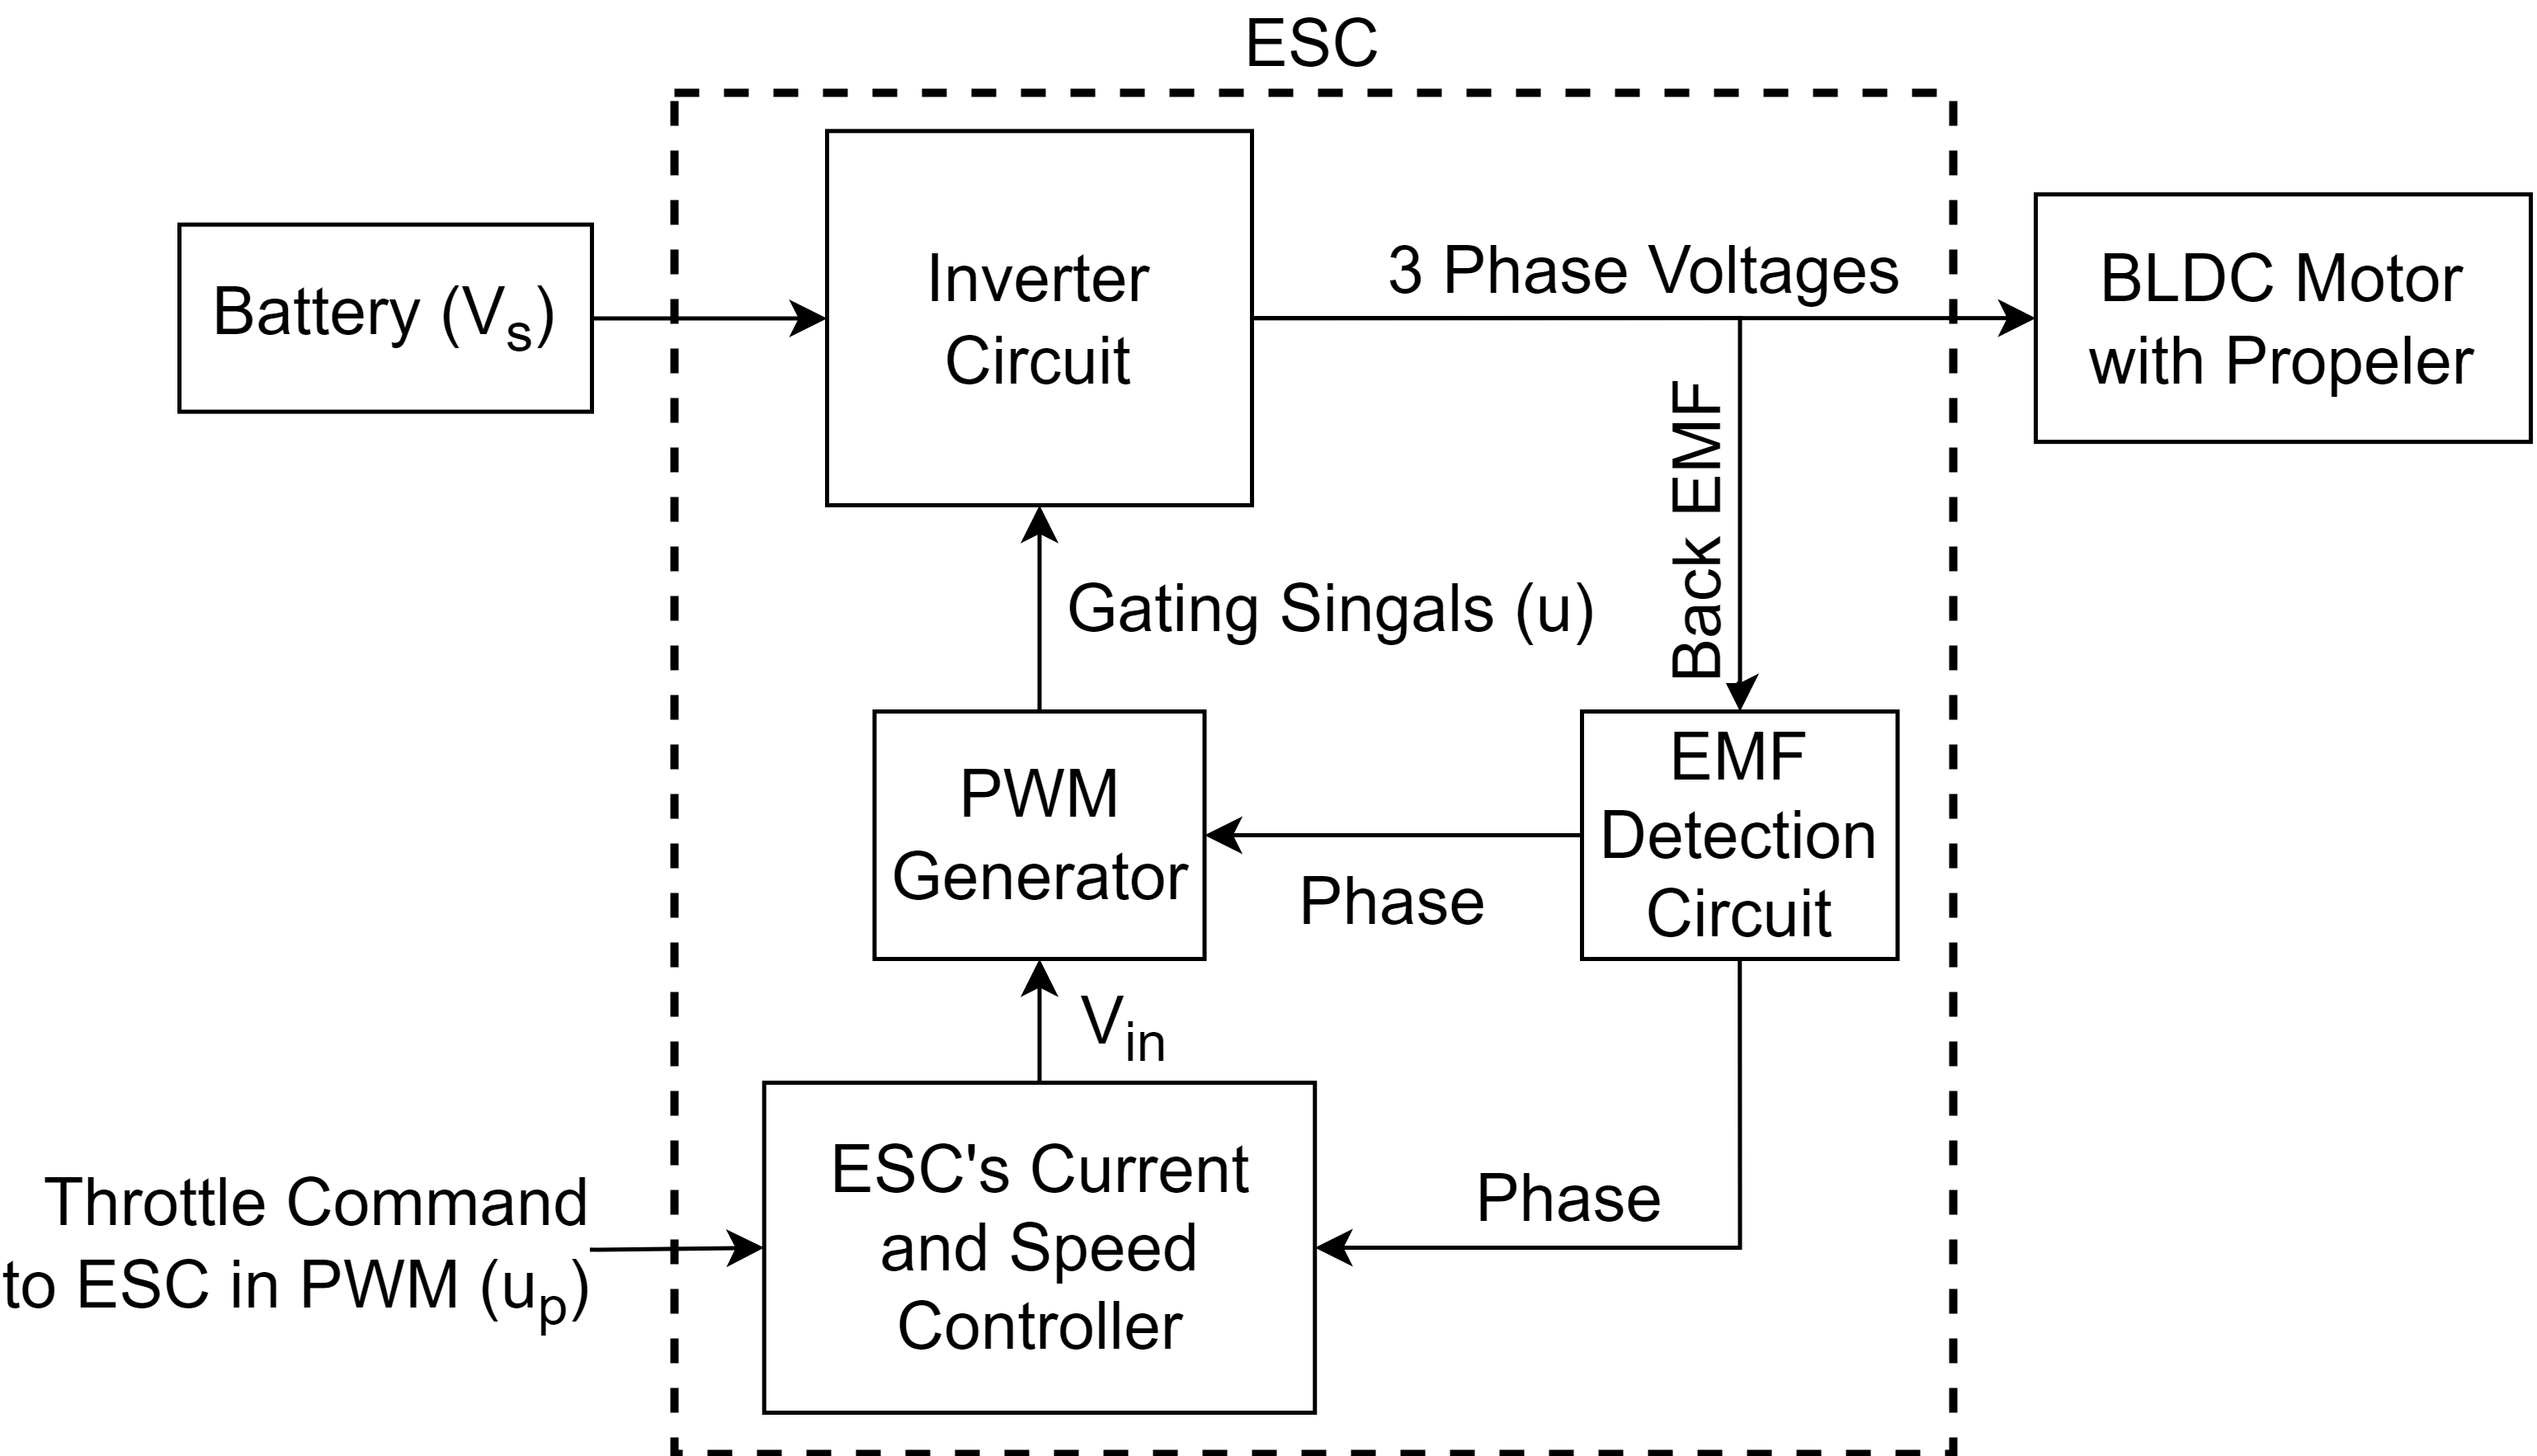
\includegraphics[width = \figsize]{./figs/figs_acc/schematic/esc_schematic.png}
    \caption{Schematic of ESC with BLDC motor}
    \label{fig::bldc_diag}
\end{figure}
%===

The motor-propeller system's function in the present context is to generate the
desired thrust $T_d$. In general this thrust is quadratic function of the
angular velocity $\omega$ of the propeller with uncertainties $(T_d = C_T
\omega_d^2 + \Delta_T)$. Let, $T (=\hat C_T \omega)$ be the thrust that has
been generated by the controller (main attitude/position control loop of the
drone) by using this thrust model and open-loop motor commands. The error in
thrust generation can be expressed as:
\begin{align*}
    e_T &= T_d - T = C_T \omega_d^2 - \hat C_T \omega^2 + 2 \Delta_T\\
        &= C_T (\omega + \omega_d) e_{\omega} + \Delta C_T \omega^2 + 2 \Delta_T
\end{align*}
Thus the thrust error $e_T$ is a function of the angular velocity error and the
uncertainties in the thrust model. Both of these errors cannot be reduced by
using attitude error feedback with limited excitation persistence. The goal of the present work is to make $e_\omega \rightarrow 0$ asymptotically
by using the RPM feedback. Such approach is expected to improve the tracking of
the thrust command ($T_d$) by reducing the thrust error ($e_T$) due to angular
velocity uncertainties and providing a linear dynamics for the actuator the can
further be used to design estimators for thrust coefficient ($C_T$)
from attitude feedback.

The proposed approach is based on a nonlinear dynamic model of the
motor-propeller system, which is identified using RPM feedback. The model is
then used to design an adaptive robust controller that can asymptotically tracks
a given reference and estimates the nonlinear model parameters in real-time. As
the RPM measurement is prone to significant noise, DCARC is used to design the
controller. The controller is then validated on a test bench.

% ==============================================================================
\newpage
\section{RPM Measurement}
Real-time angular velocity measurement involves counting commutation signals transmitted via
an auxiliary cable from the ESC. This is achieved by utilizing an interrupt
trigger to record the time elapsed since the previous commutation in an array,
which resets after a defined sampling period. This approach enhances measurement
resolution compared to counting commutations within a specific sampling period.
Let $\hat \omega_{\delta t}$ represent angular velocity measured using commutation durations
($\delta t$) and $\hat \omega_{n_C}$ denote angular velocity measured using commutation
counts ($\delta n_C$) within a sampling period \cite{PX4-autopilot-rpm}.
%===
\begin{align}
    \hat \omega_{n_C} &= \frac{2 \pi n_C}{N_p f_s} \, rad/s, \quad
    \hat \omega_{\delta t} = \frac{2 \pi}{N_p  \delta t} \, rad/s
\end{align}
Where,
\begin{align*}
    N_p &- \text{No. of pole pairs in the motor (here, 7)}\\
    f_s &- \text{Sampling frequency}\\
    \delta t &- \text{Durtion between two commutations}\\
    n_C &- \text{No. of commutations within a sampling period}
\end{align*}
%===
In both cases, the minimum angular velocity from which the measurement begins is $\omega_{min} = \frac{2 \pi}{N_p f_s}$. This is because no commutation would be registered at a speed slower than $\omega_{min}$.

Commutation duration, denoted as $\delta t$, is determined by a higher frequency counter, $f_t$, which is not bound by the overall system sampling rate. Therefore, we can express $\delta t$ as $\delta t_k / f_t$.

As for the resolution of our measurement processes:
%===
\begin{align}
    &\abs{\Delta \hat \omega_{n_C}} = \frac{2 \pi \abs{\Delta n_C} }{N_p f_s} \\
    &\implies \abs{\Delta \hat \omega_{n_C}}_{\min} =\frac{2 \pi}{N_p f_s} = \omega_{min}\\
    %===
    &\abs{\Delta\hat \omega_{\delta t}} = \frac{2 \pi \abs{\Delta \delta t}}{N_p  \delta t^2} = \frac{\abs{\Delta \delta t}}{\delta t} \hat \omega_{\delta t} = \frac{\abs{\Delta \delta t_k}}{\delta t_k} \hat \omega_{\delta t}\\
    &\implies  \abs{\Delta\hat \omega_{\delta t}}_{\min} = \frac{\abs{\Delta \delta t_k}_{\min}}{\delta t_k} \hat \omega_{\delta t} = \frac{\hat \omega_{\delta t}}{\delta t_k}
\end{align}
%===
In this setup, the resolution of $\hat \omega_{n_C}$ remains constant at $\omega_{\min}$. However, in the case of $\hat \omega_{\delta t}$, the resolution depends on the instantaneous $\omega_{\delta t}$ and the frequency of the counter, $f_t$. Using a sufficiently fast counter ensures that the $\hat \omega_{\delta t}$ measurement process achieves significantly higher resolution compared to $\hat \omega_{n_C}$.

Given that multiple measurements of $\delta t$ occur within a single sampling
instance and that the process is susceptible to noise due to interrupt skips, we
adopt a median-based approach to estimate angular velocity at the end of a given
sampling
instance. Unlike other averaging methods, using the median effectively
eliminates spikes in $\delta t$ that can occur when an interrupt is skipped.
Detailed pseudocode for this algorithm is presented in Algorithm-\ref{alg::ISR}
and Algorithm-\ref{alg::get_rpm}.

%===

\RestyleAlgo{boxruled}
\LinesNumbered
\begin{algorithm}[H]
    \scriptsize
    $n_C \peq 1$\;
    \Comment*[l]{$C_c$ - Counter value at current interrupt}
    \Comment*[l]{$P_c$ - Counter value at previous interrupt}
    $\delta t_k = C_c - P_c$\;
    \If{ $\delta t_k \leq 0$ }
        {\Comment*[l]{Correcting for integer overflow}
         $\delta t_k \peq 2^{32}$}
    $\pmb{\delta t_k} [n_C-1] =  \delta t_k$\;
    $P_c = C_c$
    \caption{\small Interrupt Service Routine}
    \label{alg::ISR}
\end{algorithm}

%===
\RestyleAlgo{boxruled}
\LinesNumbered
\begin{algorithm}[H]
    \scriptsize
    $N_p = 7$\;
    $f_t = 10^6$\;
    $M = \frac{2 \pi}{N_p} \times f_t$\;
    \eIf {$n_C > 0$ and $n_C \leq n_{C_{max}}$ and $\norm{n_C - n_{C_{old}}} \leq \delta n_{C_{max}}$}
        {\Comment*[l]{Median removes spikes in the data}
         $\omega = \frac{M}{\text{Median}(\pmb{\delta t_k})}$\;
         $ \omega_{old} = \omega$\;
         $n_{C_{old}} = n_C$\;
        }
         {$\omega = \omega_{old}$}
    $n_C = 0$
    $\pmb{\delta t_k} = \pmb 0$\;
    \caption{\small RPM Measurement Function}
    \label{alg::get_rpm}
\end{algorithm}

%===
\begin{figure}[H]
    \centering
    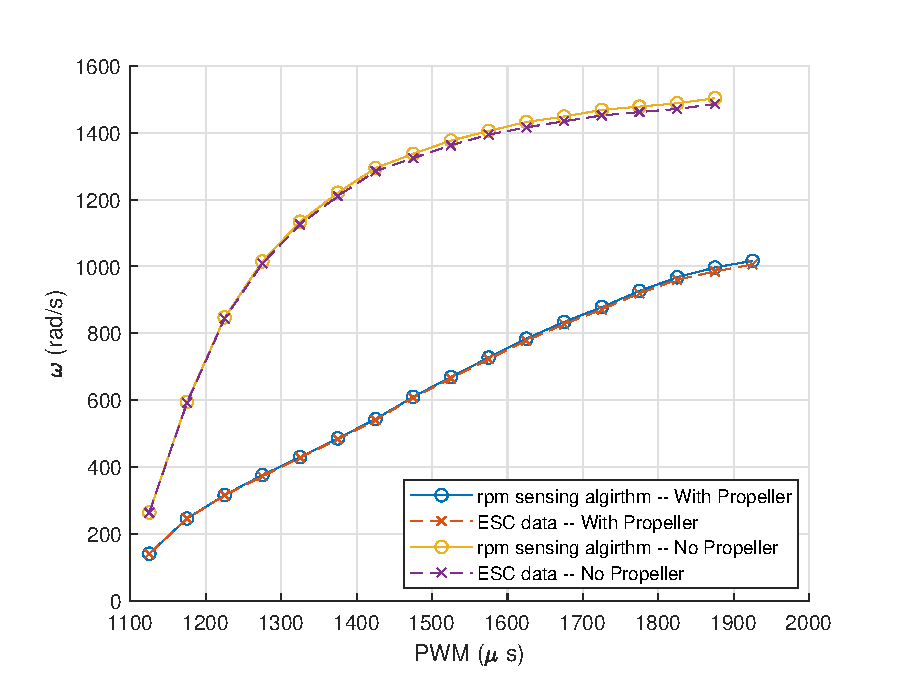
\includegraphics[width = \figsize]{./figs/figs_acc/rpm_feedback/rpm_meas.eps}
    \caption{RPM vs PWM with and without propeller}
    \label{fig::valid}
\end{figure}
%===
The measurement algorithm's validation process is conducted by comparing its results against the ESC data-log, as depicted in Fig.-\ref{fig::valid}. These validation plots not only confirm the algorithm's accuracy but also reveal the presence of non-linear input compensation mechanisms within the ESC.

%===============================================================================
\newpage
\section{Dynamic model}
The Castle Creations ESC incorporates a microcontroller that employs a non-linear scaling mechanism to transform the input PWM signal's duty cycle ($u_p$) into the duty cycle of the $24,kHz$ PWM signals sent to the inverter, thereby effectively adjusting the source voltage applied to the motor\cite{kim2017electric}. This non-linear transformation aims to achieve a linear input-to-thrust relationship, departing from the quadratic one. Consequently, the PWM input to the ESC ($u_p$) undergoes filtering through a non-linear function, denoted as $g_m$, resulting in the PWM duty-cycle input to the inverter ($u_m$). This relationship can be represented as:
%===
\begin{align}\label{eqn::esc_input}
    u_m &= g_m(u_p)\quad
    V_s = u_m V_{in} \qquad u_m \in [0, 1]
\end{align}
\begin{align*}
\text{Where,}\qquad&\\
    V_s &- \text{Effective voltage to the motor (lumped)}\\
    V_{in} &- \text{Battery voltage}
\end{align*}
%===
A constant PWM switching frequency of $400 , Hz$ is utilized, and the duty cycle is scaled accordingly with this frequency. Notably, the current ESC equipped with RPM feedback capabilities operates within the range of $1110 , \mu s$ to $1890 , \mu s$. Beyond this range, the ESC switches to a constant power mode, maintaining a constant RPM.

It's worth noting that the specific parameters governing the non-linear filter are not ascertainable with the available information. Consequently, neither $u_m$ nor $u_p$ can be considered the true input for system identification in conjunction with the propeller. To circumvent this issue, we redefine the input as the motor's angular velocity with the propeller, normalized by the input voltage ($u_\omega$). We then establish a static mapping between this quantity and the PWM input to the ESC ($u_p$).


We have speed-torque characteristics of a BLDC motor \cite{crowder2019electric}:
%===
\begin{align}
    T_e &= K_T I = K_T \frac{(V_s - E)}{R} = \frac{K_T}{R} (V_s - K_v \omega)
\end{align}
Where,
\begin{align*}
    \omega &- \text{Mechanical rpm} & &
    T_e      - \text{Electromagnetic torque}\\
    E        &- \text{Back emf} & &
    V_s      - \text{Supply voltage}\\
    I        &- \text{Total DC current}& &
    R        - \text{Total terminal phase resistance}\\
    K_T      &- \text{Motor torque constant} & &
    K_v      - \text{Kv value of the motor= $K_T$}
\end{align*}
%===
Let, $K_r = \frac{K_T}{R}$.
From (\ref{eqn::esc_input}), we have the electromagnetic torque as a function
of input and rpm:
\begin{align}\label{eqn::Te}
    T_e &= u_m K_r V_{in} - K_r K_v \omega
\end{align}
%===
We use the following quadratic relationship between propeller aerodynamic forces
and RPM \cite{pounds2010modelling}:
\begin{align}
    &\text{Propeller Thrust:}\quad
    F_T = C_{T} \omega^2\\
    &\text{Propeller moment due to drag:}\quad
    M_D = C_{D} \omega^2
\end{align}
%===
In our system, with the motor operating in a single direction, we consider
Coulomb friction as $M_f$ and damping due to viscous friction as $b_f\omega$.
We have the dynamic model of the BLDC motor with propeller using moment balance:
%===
\begin{align}
    J \dot \omega &= T_e - b_f \omega - M_f - C_D \omega^2
\end{align}
Where, $J$ is the moment of inertia. Also, let $b_m = b_f + K_rK_v$. We have the dynamic model:
\begin{equation}\label{eqn::dyn_mdl}
    J\dot \omega + b_m \omega + C_D \omega^2 + M_f = u_m K_r V_{in}
\end{equation}
%===
\subsection{Normalized Angular Velocity Input}
In the steady-state condition ($\dot \omega = 0$), (\ref{eqn::dyn_mdl}) simplifies to:
%===
\begin{align}
    &\frac{b_m}{K_r} \left(\frac{\omega_m}{V_{in}}\right) + \frac{V_{in}}{K_r} C_D \lr{\frac{\omega}{V_{in}}}^2 + \frac{M_f}{K_r V_{in}} = u_m
\end{align}
%===
We introduce a term, $u_{\omega}$, which represents the angular velocity of the motor with the propeller at unit supply voltage for the given PWM input ($u_p$). This is termed as "\textit{Normalized Angular Velocity}".
%===
\begin{align}
    u_{\omega} &= \frac{\omega}{V_{in}} \text{  at  } u_m = g_m(u_p) \\
    %===
    \implies u_m &= \underbrace{\frac{b_m}{K_r} u_\omega + \frac{\hat V_{in}}{K_r} C_D u_\omega^2 + \frac{M_f}{K_r  \hat V_{in}}}_{g_\omega (u_\omega, \hat V_{in})}
     \label{eqn::input_def}
\end{align}
where $\hat V_{in}$ is the battery voltage at calibration $(15.54\,V)$.
%===
The relationship between $u_\omega$ and $u_p$ can be estimated from the static
measurement data (Fig.-\ref{fig::norm_omega}).
%===
\begin{figure}[h]
    \centering
    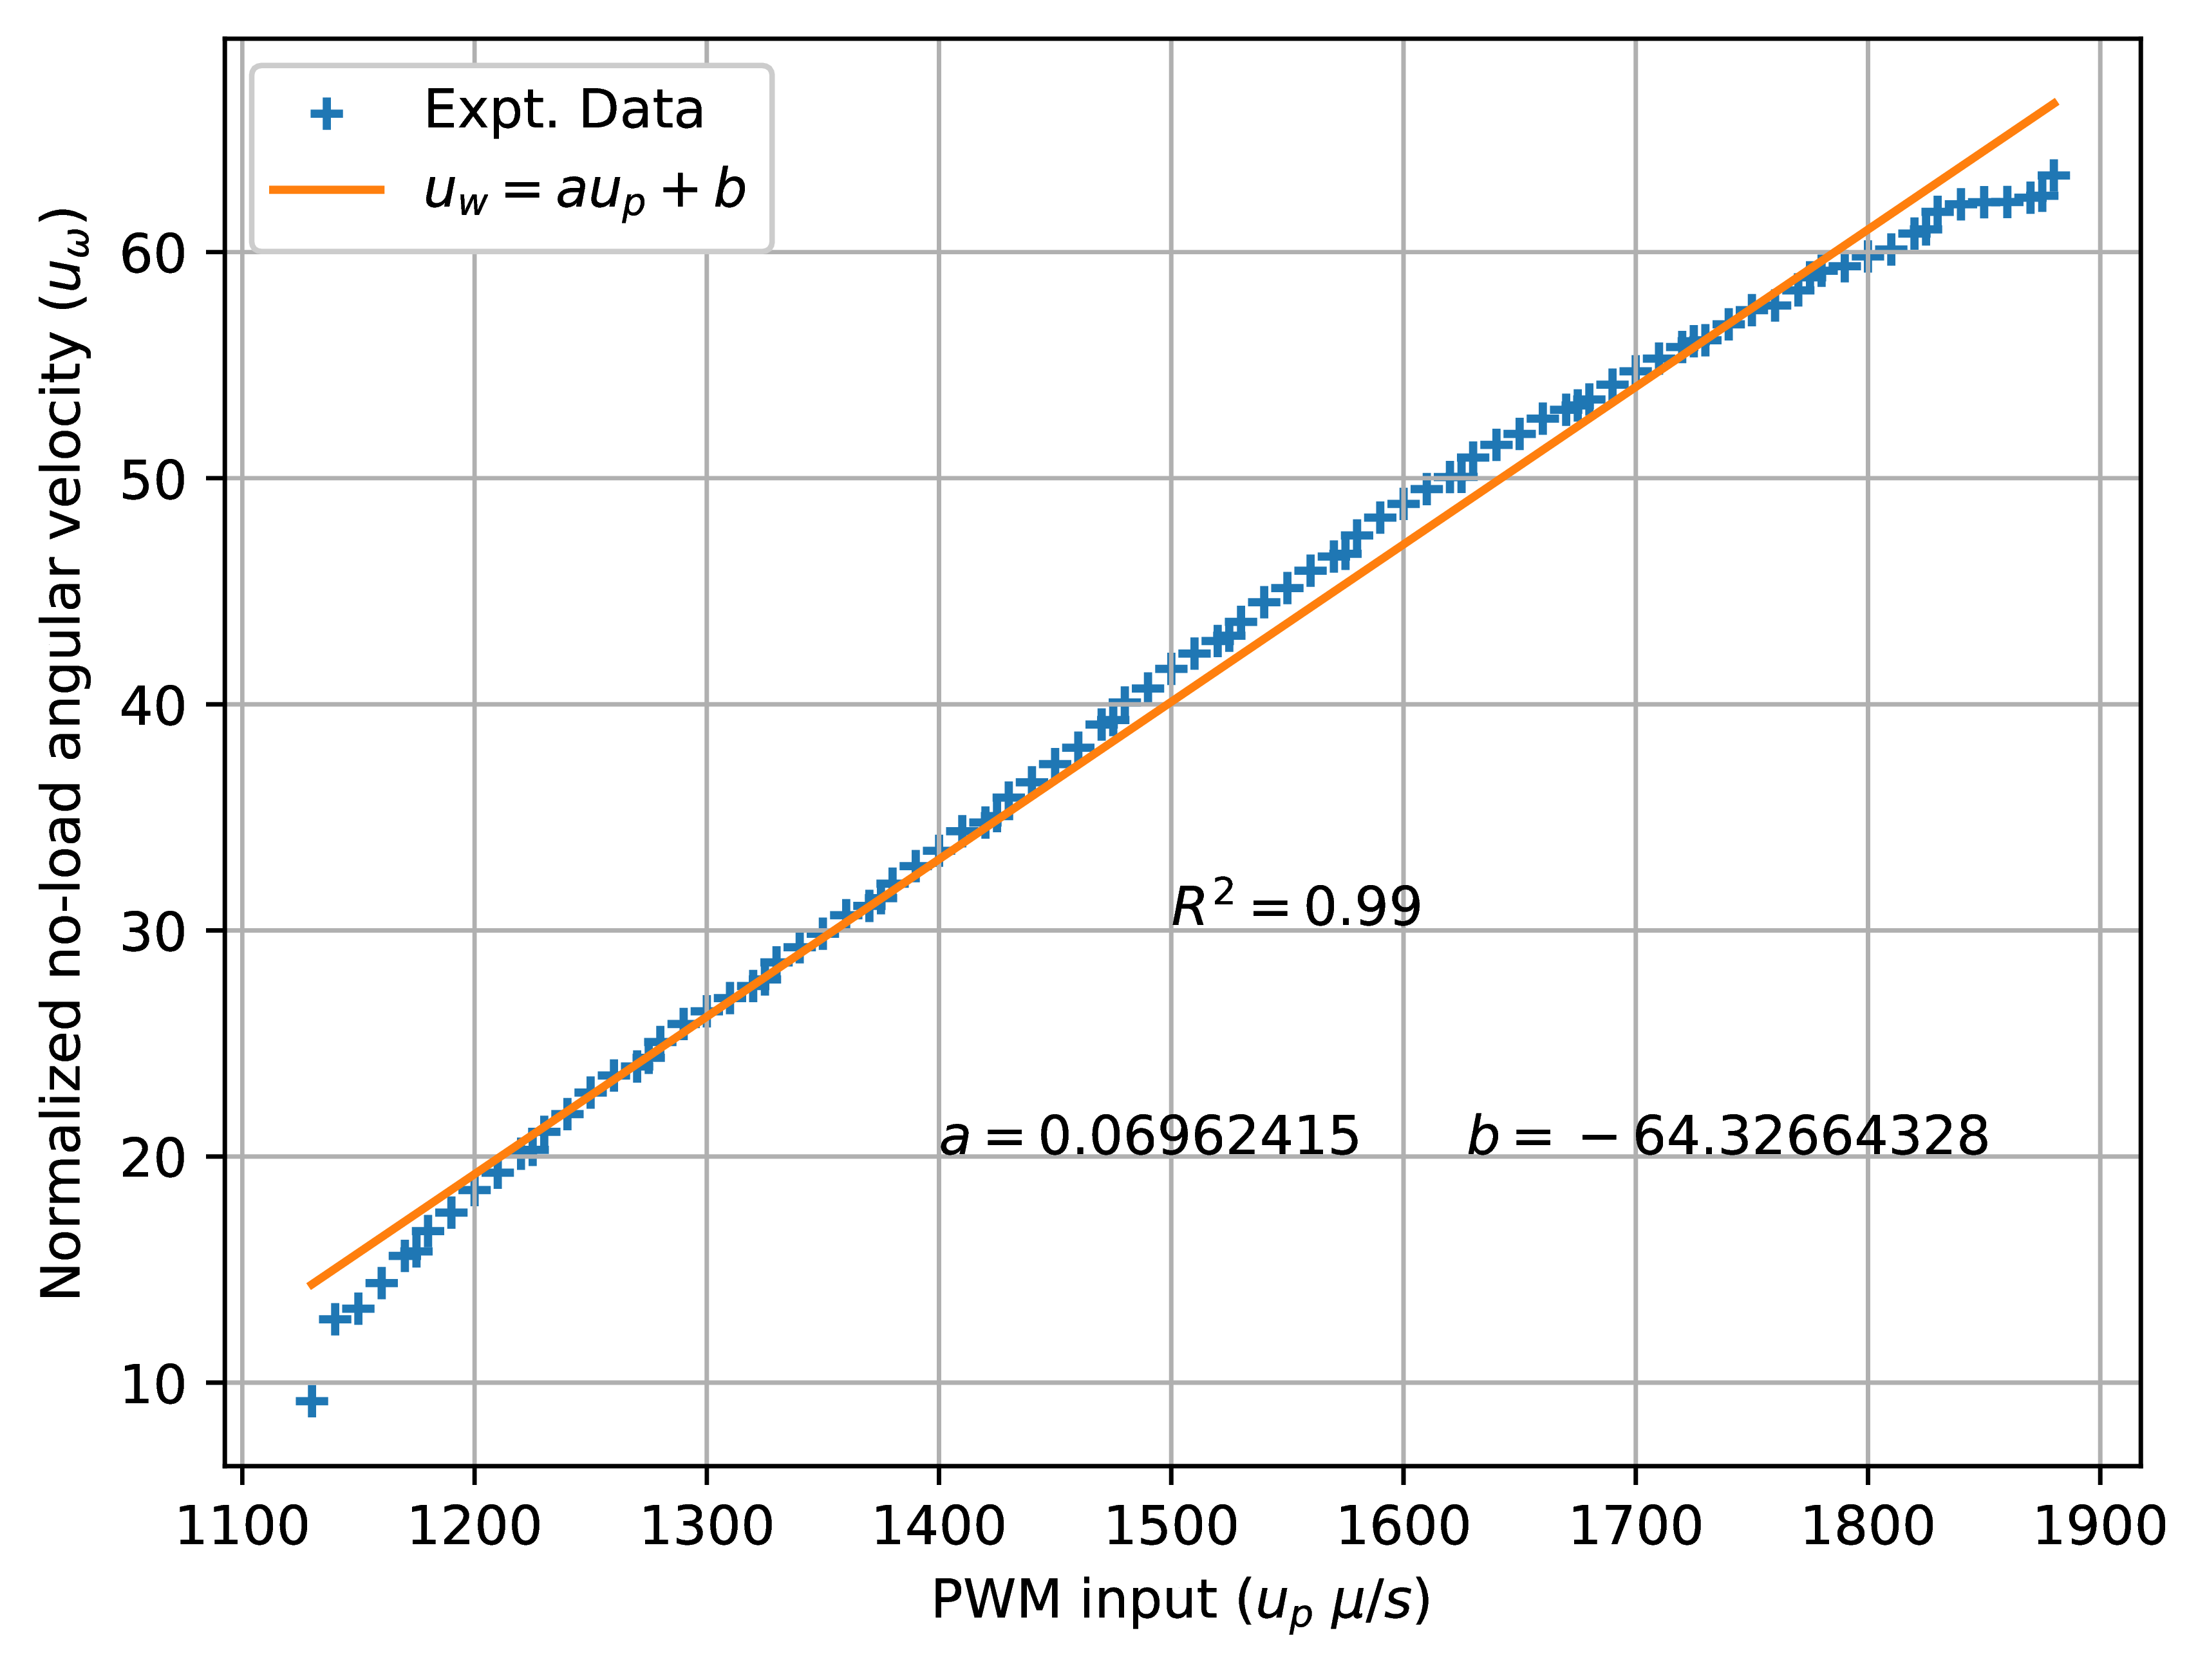
\includegraphics[width = \figsize]{./figs/figs_acc/norm_omega/no-load_rpm.png}
    \caption{$u_\omega$ as a function of $u_p$}
    \label{fig::norm_omega}
\end{figure}
%===
\begin{align}
    &u_\omega = a u_p + b
    \quad a = 0.0696
    \quad b = -64.3266   \label{eqn::uw_calib}\\
    \implies& g_m(u_p) = g_\omega(a u_p  + b, \hat V_{in})
    \; [\because u_m = g_\omega(u_\omega, \hat V_{in})]
\end{align}

%===
\subsection{Input-Output Model for Identification}
Incorporating the input definition (\ref{eqn::input_def}) into the BLDC motor model with the propeller (\ref{eqn::dyn_mdl}), we have:
%===
{\small
\begin{align}
    &J \dot \omega + b_m \omega + C_D \omega^2 + M_f \lr{1 - \frac{V_{in}}{\hat V_{in}}} = V_{in} b_m u_\omega + V_{in} \hat V_{in} C_D u_\omega^2
    \label{eqn::calib_mdl}
\end{align}
}
%===
We assume that the battery voltage remains approximately constant with small variations, which can be introduced as uncertainties:
%===
\begin{align}
    \hat V_{in} &= V_{in} ( 1 + \delta v)
    %\implies \frac{V_{in}}{\hat V_{in}} = 1 - \delta v\\
    \implies \lr{1 - \frac{V_{in}}{\hat V_{in}}} = \delta v
\end{align}
%====
This leads us to the following nonlinear input-output model with uncertainties:
\begin{equation}\label{eqn::nl_model}
    J \dot \omega + b_m \omega + C_D \omega^2 + M_f \delta v = V_{in} b_m u_\omega + V_{in}^2 (1 + \delta v) C_D u_\omega^2
\end{equation}
%===============================================================================

%===
\subsection{Model Parameter Estimates}
The model parameters and their variances are estimated using a combination of static experimental data and dynamic responses obtained under small-perturbation conditions. Subsequently, the resulting model is validated against the dynamic response of the full nonlinear model.
%===
\begin{table}[h]
    \centering
    \begin{tabular}{c l l c}
        \hline \hline
        Parameter & Value & Units & Variance ($\sigma$)            \\ \hline \hline
        $C_T$ & $7.2581 \times 10^{-06}$ & $N/(rad/s)^2$   & $4.4522 \times 10^{-8}$ \\
        $C_D$ & $3.6088 \times 10^{-08}$ & $N.m/(rad/s)^2$ & $1.3964 \times 10^{-9}$ \\
        $b_m$ & $0.0$                    & $N.m/(rad/s)$   & $4.6003 \times 10^{-6}$  \\
        $M_f$ & $1.3135 \times 10^{-3}$  & $N.m$           & $4.5277 \times 10^{-3}$ \\
        $J$   & $3.2238 \times 10^{-6}$   & $Kg.m^2$        & $7.0053 \times 10^{-6}$ \\
        \hline \hline
    \end{tabular}
    \caption{Summary of parameter estimates from static and small-perturbation experiments}
    \label{tab::parm_ests}
\end{table}

The bounds on the voltage variation based on the hard cut-off of the ESC
are found to be:
%===
\begin{align}
\abs{\delta v}_{max} = 0.2
\end{align}

Moreover, from the experiments the system start only at $u_\omega = 12.93$ which
is the minimum input required to overcome the static friction. This can be
verified as:
\begin{align}
     \lr{V_{in}^2  C_D u_\omega^2 }_{\lr{u_\omega = 12.93, V_{in} = 15.54}} = 1.4570 =  M_f
\end{align}

Thus, expanding the range of $u_w$ from $[12.93, 67.23]$ to $[0, 67.23]$, the
dynamic model \ref{eqn::nl_model} will now include the actual friction instead
of $\delta v M_f$. Rewriting \ref{eqn::calib_mdl}:

\begin{align}
    &J \dot \omega + b_m \omega + C_D \omega^2 + M_f = V_{in} \lr{b_m u_\omega + \hat V_{in} C_D u_\omega^2}
    \label{eqn::0_mdl}
\end{align}

%===
\subsection{Control form of the model}

Defining input to the system (u) as:
\begin{align}
    u &= \underbrace{\frac{1}{\hat J}\lr{\hat b_m u_\omega + \hat V_{in} \hat C_D u_\omega ^2}}_{g_u(u_\omega)} \label{eqn::uw2u}\\
    \implies u &= \frac{K_r}{J} u_m \qquad [\therefore u \geq 0] \label{eqn::ctrl_u}
\end{align}
Where $\hat \bullet$ are the estimated values of the parameters at the time of
calibration. Note that $\hat J$ is included in order to get the input into
appropriate scale.

Thus, $u$ is the actual PWM input to the inverter scaled by the ratio of the
torque constant and the winding resistance of the motor $\lr{\because K_r =
\frac{K_T}{R}}$.

Introducing the input definition (\ref{eqn::ctrl_u}) in to the nonlinear model
of the system (\ref{eqn::dyn_mdl}):
\begin{align*}
    J\dot \omega &+ b_m \omega + C_D \omega^2 + M_f = J V_{in} u\\
    \implies \dot \omega  &= -\frac{b_m}{J} \omega - \frac{C_D}{J} \omega^2 - \frac{M_f}{J} + V_{in} u\\
\end{align*}
Introducing the input and modelling uncertainties as $\Delta(u, \omega, t)$ (matched). Let,
$\bullet_{_J} = \frac{\bullet}{J}$. We have the control form of the model:

\begin{align}
   \dot \omega &= -b_{m_J} \omega - C_{D_J} \omega^2 - M_{f_J} + V_{in} u + \Delta(t, u, \omega) \label{eqn::ctrl_form}
\end{align}

\subsubsection{Input uncertainties}
The uncertainties in the input arise from the changes in the voltage from
calibration and the real system, the uncertainties in the parameter estimation
and higher-order input dynamics if any.

\subsubsection{Input to the hardware}
The control input calculated from the algorithm is not the actual hardware
input rather a nonlinear injective function of the hardware input. The
uniqueness in the mapping comes from the constraints in the range of input
values $(u > 0)$. From (\ref{eqn::uw2u}):
\begin{align*}
    &\hat V_{in} \hat C_D u_{\omega}^2 + \hat b_m u_\omega - \hat J u = 0\\
    %===
    \implies& u^{\pm}_\omega = \frac{-\hat b_m \pm \sqrt{\hat b_m ^2 + 4u \hat V_{in} \hat J \hat C_D}}{2 \hat V_{in} C_D}\\
    %===
    \because \hat b_m, \hat C_D, \hat V_{in}, \hat J &> 0 \quad \text{we have, }\qquad \\
    \implies& u^{+}_\omega = \frac{-\hat b_m + \sqrt{\hat b_m ^2 + 4u \hat V_{in} \hat J \hat C_D}}{2 \hat V_{in} \hat C_D} \geq 0 \quad \text{and} \quad
    %=
    u^{-}_\omega = \frac{-\hat b_m - \sqrt{\hat b_m ^2 + 4u \hat V_{in} \hat J  \hat C_D}}{2 \hat V_{in} \hat C_D} \leq 0 \quad \
    \forall \; u \geq 0 \\
\end{align*}
As $u_\omega > 0$ we have a unique mapping from $u$ to $u_w$:
\begin{align}
    u_\omega &= \underbrace{\frac{-\hat b_m + \sqrt{\hat b_m ^2 + 4u \hat V_{in} \hat J \hat C_D}}{2 \hat V_{in} \hat C_D}}_{g_u^+(u)}
    \label{eqn::u2uw}\\
    \implies u_p &= \frac{1}{a} \lr{g_u^+(u) - b} \qquad [\because u_\omega = a u_p + b \quad (\ref{eqn::uw_calib})]
\end{align}


%===
\newpage
\section{Actuation limits and the reference system design}
The actuator has hard limits beyond which the system doesn't function and
operational limits beyond which the system doesn't produce and useful output.
These are tabulated in the following:
\begin{table}[H]
    \centering
    \begin{tabular}{l r r r r}
        \hline \hline
        Limit & $u_p$ & $u_{\omega}$ & $u$ & $\omega$ \\ \hline \hline
        Actual Lower         & 924  & 0     & 0        & 0\\
        Lower Start          & 1110 & 12.93 & 29.08    & 200.92 \\
        Operational Lower    & 1294 & 25.74 & 115.26   & 400 \\
        Operational Higher   & 1849 & 64.35 & 720.35   & 1000\\
        Actual Higher        & 1890 & 67.23 & 786.27   &  1044.56\\
        \hline \hline
    \end{tabular}
    \caption{Input and steady state limits of the actuator}
\end{table}


% ==============================================================================

The goal of feedback control design for the actuator is two-fold:
\begin{enumerate}
\item Compensate for the input-uncertainities, un-modelled disturbances and
model-structure errors.
\item With in the operational limits, make the actuator track the response of a second-order transfer function
with no over-shoot of the form:
\begin{align*}
    G_{r}(s) &= \frac{\omega_{r}^2}{s^2 + 2s \zeta \omega_{r} + \omega_{r}^2}
    && \zeta = \frac{1}{\sqrt{2}} = 0.707
\end{align*}
Such that, $\omega_{r}$ results in the maximum possible bandwidth in presence
of uncertainties mentioned above.
\end{enumerate}

The above reference system will also introduce a limit on the maximum rate of
change of angular velocity. We have,
\begin{align*}
    &\omega(s) = \frac{\omega_{r}^2}{s^2 + 2 s \zeta \omega_{r} + \omega_{r}^2}\\
    %===
    &\text{Let,} \quad \alpha = \frac{d \omega }{dt}
    \\
    %===
    &\implies \alpha(s) = s \omega(s) =  \frac{s\omega_{r}^2}{s^2 + 2 s \zeta \omega_{r} + \omega_{r}^2}
    \\
    %===
    &\implies \norm{\alpha(j\omega)} = \norm{\frac{j \omega \omega_{r}^2}{{j \omega}^2 + 2 j \omega  \zeta \omega_{r} + \omega_{r}^2}}
    %---
    = \frac{\omega \omega_r^2}{\norm{-\omega^2 + 2 j \omega  \zeta \omega_{r} + \omega_{r}^2}}
    %---
    = \frac{\omega \omega_r^2}{\sqrt{\lr{\omega_r^2 - \omega^2}^2 + 4 \zeta^2 \omega_r^2 \omega^2}}
    \\
    %===
    &\text{as, }\quad \zeta = \frac{1}{\sqrt{2}},
    \qquad
    %===
    \norm{\alpha(j \omega)}^2 = \frac{\omega^2 \omega_r^4}{\omega^4 + \omega_r^4}
\end{align*}
% ==============================================================================

Let, $\Omega_r = \omega_r^2$, $\Omega = \omega^2$ and $M(\Omega) =
\norm{\alpha(j\omega)}^2$.
Thus, the maximum rate of change happens at:
\begin{align*}
    &\frac{d M(\Omega)}{d \Omega} = \frac{d}{d \Omega} \lr{\frac{\Omega \Omega_r^2}{\Omega^2 + \Omega_r^2}} = 0
    \quad
    %===
    \implies \frac{\Omega_r^2 \lr{\Omega^2 + \Omega_r^2} - 2 \Omega \lr{\Omega \Omega_r^2}}{\lr{\Omega^2 + \Omega_r^2}^2} = 0
    \quad
    %===
    \implies \Omega = \Omega_r
\end{align*}
Thus,
\begin{align*}
    \max \lr{{ \norm{\alpha(j \omega)}^2 }} &= M(\Omega_r) = \frac{\Omega_r^3}{2 \Omega_r^2} = \frac{1}{2} \omega_r^2
\end{align*}
\begin{equation}\label{eqn::max_bandwidth}
    \therefore \; \dot \omega_{max} = \frac{1}{\sqrt{2}} \omega_r
\end{equation}

% ==============================================================================
% ==============================================================================

\subsection{Limitations on $\dot \omega$}

The input saturation imposes limitations on the maximum and minimum rate of
change of the angular velocity $(\omega)$. From the dynamic model (\ref{eqn::ctrl_form}), removing the zero parameters
$(b_m)$ and uncertainties $(\Delta)$, we have:

\begin{align*}
    \dot \omega &= -C_{D_J} \omega^2 - M_{f_J} + V_{in} u
\end{align*}

From the above equation, we have the following bounds on the rate of change of
$\omega$, with in the operational limits [400 rad/s, 1000 rad/s].

\begin{enumerate}
    \item Maximum rate of increase:
    \begin{align*}
        \dot \omega^{+}_{max} &= -C_{D_J} (\omega_{min})^2 - M_{f_J}+ V_{in} u_{max}\\
                              &= -C_{D_J} (400)^2 - M_{f_J} + V_{in} (786.27)
                               =  10020.12 \; rad/s
    \end{align*}

    \item Minimum rate of increase:
    \begin{align*}
        \dot \omega^{+}_{min} &= -C_{D_J} (\omega_{max})^2 - M_{f_J}+ V_{in} u_{max}\\
                              &= -C_{D_J} (1000)^2 - M_{f_J} + V_{in} (786.27)
                               = 616.95 \; rad/s
    \end{align*}

    \item Maximum rate of decrease:
    \begin{align*}
        \dot \omega^{-}_{max} &= -C_{D_J} \omega_{min}^2 - M_{f_J} + V_{in} u_{min}\\
                              &= -C_{D_J} 1000^2 - M_{f_J} + V_{in} \times 0
                               = -11601.68 \; rad/s
    \end{align*}

    \item Minimum rate of decrease:
    \begin{align*}
        \dot \omega^{-}_{min} &= -C_{D_J} \omega_{min}^2 - M_{f_J} + V_{in} u_{min}\\
                              &= -C_{D_J} 400^2 - M_{f_J} + V_{in} \times 0
                               = -2198.51 \; rad/s
    \end{align*}
\end{enumerate}

% ==============================================================================

In order for the motor-propeller system to accurately track the response of a linear second-order system within the given input constraints, the maximum rate of change of the reference system state should be lower than the minimum rate of change in the actual system. This ensures that the system can keep up with the desired changes in the reference signal.

\begin{align}
    \abs{\dot \omega_{max}} &\leq \abs{\dot \omega^{+}_{min}} \label{eqn::dot_omega_max}\\
    \implies \frac{1}{\sqrt{2}} \omega_r &\leq 616.95 \; rad/s
    \qquad [\because \ref{eqn::max_bandwidth}]\\
    \therefore \omega_r &\leq  872.5 \; rad/s
    \label{eqn::omega_r_lim}
\end{align}

% ==============================================================================
% ==============================================================================

\subsection{Sampling Limitations}
The sampling due to the implementation of feedback would introduce its own
limitations on the maximum bandwidth of the reference system, namely, the
Nyquist frequency $(n_f)$ of sampling. The approximate inequality would be:
\begin{align}
    \omega_r < 2 \pi n_f
    \label{eqn::wr_lim_nf}
\end{align}

For the current set-up, $n_f = 250/2 = 125 \; Hz$. Thus,
\begin{align}
    \omega_r < 2\pi \times 125 = 785.4 \; rad/s
\end{align}

The above limit is less restrictive than the limit on the maximum rate of change
due to the passive dissipative forces on the actuator.


\bigskip \itbf{Note:} The above inequality (\ref{eqn::wr_lim_nf}), can be
flipped and combined with (\ref{eqn::dot_omega_max}) for using it as a design
limitation for the sampling system. Thus, the minimum sampling the requirement
for obtaining the maximum performance from the system as:

\begin{align}
    n_f > \frac{\abs{\dot \omega^{\pm}_{min}}}{2 \pi}
\end{align}


% ==============================================================================
% ==============================================================================

\subsection{Reference system design}
From the above inequalites on $\omega_r$, (\ref{eqn::wr_lim_nf}),
(\ref{eqn::omega_r_lim}), a conservative choice or $\omega_r$ is used for the
reference system design.

\begin{align}
    \omega_r &= 700 \; rad/s\\
    \zeta &= \frac{1}{\sqrt{2}}
\end{align}

Thus,
\begin{align}
    G_r (s) &= \frac{\omega_r^2}{s^2 + s \omega_r \sqrt{2}  + \omega_r^2}
\end{align}

% ==============================================================================
% ==============================================================================

\subsection{Discrete implementation of the reference system}

The state space representation of the reference system is:
\begin{align}
    \bm{\dot x \\ \ddot x} &= \underbrace{\bm{0 & 1 \\ -\omega_r^2 & -\sqrt{2} \omega_r}}_{A_r} \bm{x \\ \dot x} + \underbrace{\bm{0 \\ 1}}_{B_r} u
\end{align}
The discrete implementation of the above system will be of the form:
\begin{align}
    \bm{x[k+1] \\ \dot x[k+1]} &= A_d \bm{x[k] \\ \dot x[k]} + B_d u[k]\\
    %==
    A_d &= e^{A_r T} =
    e^{-\alpha T} \bm{\cos \lr{\alpha T} + \sin \lr{\alpha T} & \frac{1}{\alpha}
                        \sin \lr{\alpha T}\\
                       -2 \alpha \sin \lr{\alpha T} & \cos \lr{\alpha T} - \sin \lr{\alpha T}}
    \qquad \lrb{\alpha = \frac{\omega_r}{\sqrt{2}}}\\
    %===
    B_d &= \int_0^T e^{A_r \tau} B_r d\tau = \bm{\frac{1}{2 \alpha^2} \lrb{1 - e^{-\alpha T} \lr{\cos \lr{\alpha T} + \sin \lr{\alpha T}}} \\
    %---
    \frac{1}{\alpha} e^{-\alpha T} \sin \lr{\alpha T}}
\end{align}

% ==============================================================================
\newpage
\section{Direct compensation adaptive robust control (DCARC) design}

\subsection{Review of ARC design}

%===============================================================================
\subsection{Control form and parameter bounds for the model}

Rewriting the (\ref{eqn::ctrl_form}) with the following definitions:
\begin{align}
    \text{Let, }\quad &\Delta(t, x, u) = d_0 + d(t, x, u) \\
    %===
    \therefore \dot x &= -C_{D_J} x^2 -b_{m_J} x - M_{f_J} + d_0 + V_{in} u + d(t, x, u) \\
    %===
    \text{Let, } \quad & \theta_1 = C_{D_J} \quad \theta_2 = b_{m_J} \quad \theta_3 = M_{f_J} - d_0  \quad \text{and} \quad b = V_{in}\\
    %===
    \text{Thus, }\quad & \dot x = \underbrace{-\theta_1 x^2 -\theta_2 x - \theta_3}_{f(t, x)} + b u + d(t, x, u)
    \label{eqn::prm_ctrl_form}
\end{align}

Defining the following regression and parameter vectors:
\begin{align}
    \phi(x) &= \bm{ -x^2 & -x & -1}^T \\
    %===
    \theta &= \bm{\theta_1 & \theta_2 & \theta_3}^T = \bm{C_{D_J} & b_{m_J} & M_{f_J}-d_0}^T \\
    %===
    \text{Thus, }\quad f(t, x) &= \phi(x)^T \theta\\
    %===
\end{align}

From experimental observations \ref{tab::parm_ests}, the $2\sigma$ variation of
the parameters is about $10\%$ variation of the parameters. This is used to
compute the parameter bounds. The physics dictates that
all the physical parameters have a non-negative value. The bounds on input
uncertainties are calculated based on the maximum and minimum values of the
parameter estimates at the calibration time (same as at realtime). From (\ref{eqn::ctrl_u}):
\begin{align*}
    \abs{\Delta}_{max} &\leq \tilde \theta_{2M} \abs{u_\omega}_{max} + \lr{\tilde b_M \abs{\theta_1}_{max} + \abs{b}_{max} \tilde \theta_{1M}}\abs{u_\omega}_{max}^2  < 350 = d_M\\
    %===
    \text{where, }\quad \tilde \bullet_M &= \abs{\bullet_{max} - \bullet_{min}}\\
    %===
    \implies \abs{d_0} &\leq d_M = 350 \\
    \implies \abs{d(t)} &\leq 2 d_M = 700
\end{align*}



The following table gives the minimum, maximum and nominal values of the parameters of the equation (\ref{eqn::prm_ctrl_form}):

\begin{table}[H]
    \centering
    \begin{tabular}{r r r r}
        \hline \hline
        Parameter &Nominal & Minimum & Maximum \\ \hline \hline
        $\theta_1$            &
        $0.0112$              &
        $0.0101$              &
        $0.0123$

        \\
        $\theta_2$               &
        $0$                      &
        $0$                      &
        $1$
        \\
        $\theta_3$                 &
        $407.44$                   &
        $0$                        &
        $750$
        \\
        $b$                        &
        $15.54$                    &
        $14.5$                     &
        $16.5$
        \\
        $d(t)$                   &
        $0$                      &
        $-700$                   &
        $700$
        \\
        \hline \hline
    \end{tabular}
    \caption{Summary of parameter bounds}
    \label{tab::parm_bounds}
\end{table}

%===============================================================================
\subsection{Desired model compensation input}
The role of model compensation is to generate the required input for the
nominal plant state $(x)$ to track the desired trajectory $(x_d)$.

Let,
\begin{align}
    z &= x - x_d\\
    \implies \dot z &= \dot x - \dot x_d\\
    \implies \dot z &= \phi^T \theta +  bu + d - \dot x_d \qquad \lrb{\because \ref{eqn::prm_ctrl_form}}
    \label{eqn::error_dyn}
\end{align}

Considering only the nominal dynamics, i.e., assuming zero uncertainties ($d = 0$), the error dynamics can be simplified as follows:

\begin{align}
    \dot z &= \phi^T \theta + bu - \dot x_d
    \label{eqn::nom_error_dyn}
\end{align}

The total control input $u$ can be decomposed into $u_m$ (model compensation input) and $u_s$ (robust control input).

\begin{align}
    u &= u_m + u_s
\end{align}

The model compensation input in the present case is derived solely from the
reference trajectory dynamics and the model parameters. We have,
\begin{align}
    u_m &= \frac{1}{\hat b} \lr{\dot x_d - \phi^T(x_d) \hat \theta}
         = \frac{1}{\hat b} \lr{\dot x_d - \phi^T_d \hat \theta}
         \qquad \lrb{\text{where, } \phi_d  = \phi(x_d)}
\end{align}

Substituting the above expression for $u_m$ in the nominal error dynamics (\ref{eqn::nom_error_dyn}), we get:

\begin{align*}
    \dot z &= \phi^T \theta + b \lr{u_s + u_m} - \dot x_d \\
    %===
    &= \phi^T \theta + bu_s + \lr{b - \hat b} u_m  + \hat b u_m - \dot x_d \\
    %===
    &= \phi^T \theta - \phi^T_d \hat \theta + bu_s - \tilde b u_m
    &&\lrb{\text{Let, } \tilde b = \hat b - b}\\
    %===
    &= \phi^T \theta - \phi^T_d \theta + \phi^T_d \theta - \phi^T_d \hat \theta + bu_s - \tilde b u_m\\
    %===
\end{align*}
Let, $\tilde \phi = \phi(x) - \phi(x_d)$ and $\tilde \theta = \hat \theta -
\theta$. The error dynamics can be rewritten as:
\begin{align}
    \dot z &= \tilde \phi^T \theta - \phi^T_d \tilde \theta + bu_s - \tilde b u_m \label{eqn::error_dyn_model_comp}
\end{align}

It can be noted that as $\theta$ is unknown with known bounds, there exists a
known function $\delta_\phi(x, t)$ such that:
\begin{align}
    \abs{\tilde \phi^T \theta} &\leq \delta_\phi(x, t) \abs{z}
    \label{eqn::tl_phi_bound}
\end{align}


Further, let:
\begin{align}
    \phi_{du}^T &= \bm{\phi_d^T & u_m}\\
    \theta_{b} &= \bm{\theta^T & b} \qquad \implies \tilde \theta_b = \bm{\tilde \theta^T & \tilde b}
\end{align}

Substituting the above definitions in (\ref{eqn::error_dyn_model_comp}), we get:
\begin{align}
    \dot z &= \tilde \phi^T \theta - \phi_{du}^T \tilde \theta_b + bu_s
    \label{eqn::error_dyn_model_comp_2}
\end{align}

The robust feedback control input $u_s$ is further decomposed into two parts:
\begin{align}
    u_s &= u_{s1} + u_{s2}\\
    u_{s1} &= - k z
\end{align}

Substituting above expression for $u_s$ in the error dynamics
(\ref{eqn::error_dyn_model_comp_2}), we get:

\begin{align}
    \dot z + bk z &= \tilde \phi^T \theta - \phi_{du}^T \tilde \theta_b + bu_{s2}
    \label{eqn::error_feedback_dyn}
\end{align}

The robust feedback control input $u_{s2}$ is designed to account for the model
structure and input uncertainties (d) which are assumed to be zero in this
design. Thus analyzing the error dynamics (\ref{eqn::error_feedback_dyn}) with
$u_{s2} = 0$:

\begin{align*}
    \dot z + bk z &= \tilde \phi^T \theta - \phi_{du}^T \tilde \theta_b
\end{align*}

If $\tilde \theta_b$ asymptotically becomes zero, then the feedback gain of the
error dynamics should be large enough to compensate for $\tilde \phi^T \theta$.
From (\ref{eqn::tl_phi_bound}), we get the following condition for the zero
tracking error when the parametric uncertainties are zero:
\begin{align}
    bkz &\geq \delta_\phi(x, t) \abs{z}\\
    C1: \qquad \implies k &\geq \frac{1}{b}\delta_\phi(x, t) > \frac{1}{\hat b_{min}} \delta_\phi(x, t)
    \label{eqn::k_bound}
\end{align}

%===============================================================================
\subsection{Discontinuous projection based adaptation law}
The parameter estimation error $\tilde \theta_b$ can be reduced to zero asymptotically by using a gradient-based parameter adaptation law. This adaptation law is defined as follows:
\begin{align}
    \dot{\hat{\theta_b}} &= Proj_{\hat{\theta_b}}\lr{\Gamma \phi_{du}(t) z}
\end{align}
Where $\Gamma$ is a positive definite, diagonal adaption rate matrix.
We define, \itbf{Discontinuous projection mapping} $Proj()$ for a vector as follows:
\begin{align}
    Proj_{\hat{\theta}} (\bullet) &= \bm{Proj_{\hat \theta_1}(\bullet_1), &
                                        Proj_{\hat \theta_2}(\bullet_2), &
                                        \hdots, &
                                        Proj_{\hat \theta_n}(\bullet_n)}\\
    Proj_{\hat \theta_i}(\bullet_i)
    &= \begin{cases}
        0 & \text{if } \begin{cases}
                        \hat \theta_i &= \hat \theta_{i_{min}} \text{  and  } \bullet_i < 0\\
                        \hat \theta_i &= \hat \theta_{i_{max}} \text{  and  } \bullet_i > 0\\
                       \end{cases}\\
        \bullet_i & \text{otherwise}
    \end{cases}
\end{align}
The above mapping has the following properties:
\begin{itemize}
    \item[$P_1$:]
    \begin{align}
        \hat{\pmb \theta} \in \bar \Omega_{\theta}=\{\hat{\pmb \theta} :
        \theta_{i_{min}} \leq \hat \theta_i \leq \theta_{i_{max}} \; \forall
        i\} \; \forall t
    \end{align}

    \item[$P_2$:]
    \begin{align}
        \tilde{\pmb{\theta}} \left[ \Gamma^{-1} Proj_{\hat{\pmb\theta}}
        \lr{\Gamma \pmb \phi z} - \phi z \right] \leq 0 \: \forall t \qquad
        [\tilde{\pmb{\theta}} = \hat{\pmb\theta} - \pmb \theta]
    \end{align}
\end{itemize}

The above adaptation low asymptotically reduces the errors due to parameter
estimation to zero. This can be proved by adding the following positive
definite term to the lyapunov function:
\begin{align*}
    \tilde \theta_b^T \Gamma^{-1} \tilde \theta_b
\end{align*}
%===============================================================================
%===============================================================================

\subsection{Proof of stability and tracking performance when $d = 0$}

When $d = 0$ consider the following Lyapunov function:
\begin{align*}
    V &= \frac{1}{2} z^2 + \frac{1}{2} \tilde{\theta}_b^T \Gamma^{-1} \tilde{\theta}_b\\
    %===
    \implies \dot V &= z \dot z + \tilde \theta_b^T \Gamma^{-1} \dot{\hat \theta}_b\\
    %===
    &= z \lr{- bk z +  \tilde \phi^T \theta - \phi_{du}^T \tilde \theta_b}+ \tilde \theta_b^T \Gamma^{-1} \dot{\hat \theta}_b\\
    %===
    &\leq -bkz^2 + \delta_\phi z^2 - \tilde \theta_b^T \phi_{du} z + \tilde \theta_b^T \Gamma^{-1} \lr{\Gamma \phi_{du} z}\\
    %===
    &\leq z^2 \lr{-bk + \delta_\phi} < 0 \qquad \lrb{\because (\ref{eqn::k_bound})}\\
    \implies \dot V &< 0
\end{align*}
Thus,
\begin{itemize}
    \item $\dot V$ is negative semi-definite.
    \item $V$ has a lower bound $ \lrb{\because \geq 0}$.
\item $\dot V$ is uniform continuous $\lrb{\because \ddot V \leq \lr{-bk +
\delta_\phi}z \dot z }$.
    \item $\therefore$ For a bounded $x_d$, $z \in L_\infty$, $\tilde{
    \theta}_b \in L_{\infty}$ and $\dot z \in L_\infty$, $\ddot V \in L_\infty$.
\end{itemize}

Hence, the parameter estimates and tracking errors are bounded, and the system
is stable.

Also, since $V$ is non-decreasing and positive definite,
\begin{align*}
    V(0) - V(t) &\leq V(0) \quad
    \implies -\int_0^t V d \tau \leq V(0)\\
    \implies \int_0^t \lr{-bk + \delta_\phi} z^2 d \tau &\leq V(0)\\
    \implies \sqrt{\int_0^t \norm{z}^2 d \tau } &\leq \sqrt{\frac{2 V(0)}{\lr{-bk + \delta_\phi}}} \leq \infty\\
    \therefore z &\in L_2
\end{align*}
From Barbalat's lemma, we have,
\begin{align*}
    \dot V \rightarrow 0 \quad z \rightarrow 0 \quad \text{as} \quad t \rightarrow 0
\end{align*}
Thus the parameter estimates are bounded, and the tracking error asymptotically
goes to zero as  $t \rightarrow 0$.

%===============================================================================
\subsection{Robust feedback control design}

Adding model uncertainties to the error dynamics (\ref{eqn::error_feedback_dyn}):
\begin{align}
    \dot z + bk z &=  \tilde \phi^T \theta + bu_{s2} - \lrb{ \phi_{du}^T \tilde \theta_b - d}
    \label{eqn::error_feedback_dyn_uncertain}
\end{align}

The left side of (\ref{eqn::error_feedback_dyn_uncertain}) represents the
stable nominal closed-loop dynamics. The terms in the brackets of the right
hand side represents the effect of all model uncertainties. Though these terms
are unknown, but they are bounded above with some known function h(x, t). The
goal of the robust feedback is to account for the uncertainties during the
transients and the steady state of parameter adaptation. Thus, $u_{s2}$ is
synthesized to satisfy the following two conditions:
\begin{align}
    C2:& \qquad z \lrb{-\phi_{du}^T \tilde \theta_b + d + b u_{s2}} \leq \varepsilon \\
    C3:& \qquad z b u_{s2} \leq 0
\end{align}

%===============================================================================

The function $h(x, t)$ is calculated as follows:

\begin{align}
    \abs{\phi_{du}^T \tilde \theta_b - d} &\leq h\\
    \implies h(x_d, t) &= \abs{\phi_{du}^T(x_d, t)}  \tilde \theta_{bM} + 2 d_M \qquad \lrb{\because d \leq 2d_M }
\end{align}

The robust feedback control input $u_{s2}$ is thus designed to satisfy the conditions $C2$ and $C3$ as follows:
\begin{align}
    u_{s_2} &= -\frac{1}{\hat b_{min}} S(h \sign(z)) \label{eqn::robust_u}\\
    %===
    \text{Where,  } \qquad
    S(h \sign(z)) &= h \sat \lr{ \frac{h}{4 \varepsilon} z} &[\text{Smoothing function}]\\
    %===
    \sat (x) &= \begin{cases}
        x  & \text{if  } \abs{x} \leq   1\\
        \sign(x) &  \text{otherwise}
    \end{cases}
\end{align}

The above defined smoothing function, $S(.)$, has the following properties:

\begin{itemize}
\item[$P_3$:]
\begin{align}
    z S(h \sign(z)) = z h \sat \lr{\frac{h}{4 \varepsilon} z} \geq 0
\end{align}
$\because$ $z$ and $\sat \lr{\frac{h}{4 \varepsilon} z}$ have the same sign.

\item[$P_4$:]
\begin{align}
    z \left[h \sign(z) - S(h\sign(z)) \right] \text{  is bounded.}
\end{align}
\itbf{proof:}
\begin{align*}
    z \left[h \sign(z) - S(h\sign(z)) \right] &= z \left[h \sign(z) - h \sat \lr{\frac{h}{4 \varepsilon} z} \right]
\end{align*}

\begin{enumerate}
\item Outside the boundary layer, i.e., $\lr{\abs{z} > \frac{4 \varepsilon}{h}
}$:
\begin{align*}
    zh \sign(s) - z h \sat \lr{\frac{h}{4 \varepsilon} z} &= h \abs{z} - h\abs{z} = 0
\end{align*}

\item Inside the boundary layer, i.e., $\lr{\abs{z} < \frac{4 \varepsilon}{h}}$
\begin{align*}
    zh \sign(z) - z h \sat \lr{\frac{h}{4 \varepsilon} z} &= h \abs{z} - \frac{h^2}{4 \varepsilon} z^2\\
    &= \varepsilon - \left[ \frac{1}{2 \sqrt{\varepsilon}} h \abs{z} - \sqrt{\varepsilon} \right]^2\\
    &\leq \varepsilon\\
\end{align*}
\end{enumerate}
\end{itemize}

The rubust control input definition (\ref{eqn::robust_u}) satisfies the
conditions $C2$ and $C3$ as following:
\begin{enumerate}
    \item[C2:]
    \begin{align*}
        z b u_{s2} &= -z \lr{\frac{b}{\hat b_{min}}} S(h \sign(z)) < 0
        \qquad \lrb{\because \frac{b}{b_{min}} > 1} \\
    \end{align*}
As the input gain doesn't change sign, the above inequality is always satisfied.

    \item[C3:]
    \begin{align*}
        z \lrb{-\phi_{du}^T \tilde \theta_b + d + b u_{s2}} &= z \lrb{-\phi_{du}^T \tilde \theta_b + d - \delta b S(h \sign(z))} \qquad \lrb{\text{where, } \quad \delta b = \frac{b}{\hat b_{min}} \geq 1 }\\
        %===
        &\leq z \lrb{h(x_d, t) - \delta b S(h \sign(z))}\\
        %===
        &\leq z \lrb{h(x_d, t) - S(h \sign(z))} \leq \varepsilon
        \qquad [\because \text{Property } P_4]
    \end{align*}

\end{enumerate}

\subsubsection{Proof of stability and tracking performance}
Consider the following Lyapunov function:
\begin{align*}
    V &= \frac{1}{2} z^2\\
    \implies \dot V &= z \dot z = z \lr{-kbz + \tilde \phi^T \theta - \phi_{du}^T \tilde \theta_b + d + b u_{s2}}\\
    %===
    &= -(kb - \delta_{\phi})z^2 + z \lr{- \phi_{du}^T \tilde \theta_b + d + b u_{s2}}\\
    &\leq -(kb - \delta_{\phi}) z^2 + \varepsilon \qquad [\because C3] \\
    \implies \dot V &\leq -k_p z^2 + \varepsilon = - 2 k_p V + \varepsilon \qquad \lrb{\text{where } k_p = kb - \delta_{\phi} > 0}
\end{align*}
By applying comparison lemma, the upper bound can be found from the forced
response of the following ODE:
\begin{align*}
    &\dot V + 2 k_p V = \varepsilon\\
    &\implies sV - V(0) + 2 k_p V = \varepsilon\\
    &\implies V = \frac{V(0)}{s + 2 k_p} + \frac{\varepsilon}{2 k_p}\\
    &\implies V(t) = V(0)e^{2 k_p t} + \int_0^t{e^{2 k_p (t-\tau)} \varepsilon(\tau) d\tau}\\
    &\implies \frac{1}{2} z^2 = \frac{1}{2} z(0)^2 e^{2 k_p t} + \int_0^t{e^{2 k_p (t-\tau)} \varepsilon(\tau) d\tau}\\
    %===
    &\implies \abs{z(t)}^2 = z(0)^2 e^{2 k_p t} +2 \int_0^t{e^{2 k_p (t-\tau)} \varepsilon(\tau) d\tau}\\
    &\qquad \qquad \leq z(0)^2 e^{2 k_p t} + \frac{\varepsilon_M}{k_p} \left[1 -  e^{2 k_p t} \right]
    %==
\end{align*}
This the system is stable, and the transient response is bounded that
exponentially converges to $\frac{\varepsilon}{k_p}$.

%===============================================================================
\subsection{Controller parameter selection and tuning}
\subsubsection{Adaptation rate tuning}
\subsubsection{Robust feedback gain tuning}


% %===============================================================================
\newpage
\bibliographystyle{unsrt}
\bibliography{refs}

\end{document}
